\documentclass{beamer}
\mode<presentation>
{
  \usetheme{Berkeley}
  \setbeamertemplate{footline}[frame number]
  \setbeamercovered{transparent}
}
\usepackage[english]{babel}
\usepackage[latin1]{inputenc}
\usepackage{times}
\usepackage[T1]{fontenc}
\usepackage{tikz}
\usepackage{booktabs}
\usepackage{multicol}
\usepackage{listings}
\usepackage[binary-units=true]{siunitx}
\usepackage{amsmath}
\usepackage{underscore}
\usepackage{bbding}
\definecolor{lstpurple}{rgb}{0.5,0,0.35}
\definecolor{lstred}{rgb}{0.6,0,0}
\definecolor{lstgreen}{rgb}{0.25,0.5,0.35}
\definecolor{lstblue}{rgb}{0.25,0.35,0.75}
\def\linlinep{\lstinline[basicstyle=\ttfamily,language=python]}
\def\linlinec{\lstinline[basicstyle=\ttfamily,language=c++]}
\newcommand\supertiny{\fontsize{3.5pt}{4.2}\selectfont}
\lstdefinelanguage{cython}[]{python}{morekeywords={
    cdef, cimport, cppclass, extern, namespace}}
\lstdefinelanguage[extra]{python}[]{python}{
    morekeywords=[2]{bytes, yield, unicode},
    moredelim=*[is][\textcolor{red}]{$}{$}
}
\lstset{language = [extra]python,
    showstringspaces = false,
    columns = flexible,
    basicstyle = \ttfamily\footnotesize,
    keywordstyle = \color{lstpurple},
    keywordstyle = [2]\color{lstblue},
    commentstyle = \color{lstgreen},
    stringstyle = \color{lstred},
    numbers=left,numberstyle=\tiny,numbersep=1ex
}
\lstdefinelanguage[extra]{c++}[]{c++}{
    moredelim=*[is][\textcolor{red}]{$}{$}
}
\title[Boost.Python]{How I Learnt To Stop Worrying And Love Boost.Python}

\subtitle{An adventure in high-performance networking}

\author{Bruce Merry}
% - Give the names in the same order as the appear in the paper.
% - Use the \inst{?} command only if the authors have different
%   affiliation.

\institute[SKA SA]{SKA South Africa}

\date{PyCon ZA 2015}

% If you have a file called "university-logo-filename.xxx", where xxx
% is a graphic format that can be processed by latex or pdflatex,
% resp., then you can add a logo as follows:

\pgfdeclareimage[height=1cm]{logo}{ska-africa.jpg}
\logo{\pgfuseimage{logo}}



\AtBeginSubsection[]
{
  \begin{frame}<beamer>{Outline}
    \tableofcontents[currentsection,currentsubsection]
  \end{frame}
}


% If you wish to uncover everything in a step-wise fashion, uncomment
% the following command: 

%\beamerdefaultoverlayspecification{<+->}


\begin{document}

\begin{frame}
  \titlepage
\end{frame}

\begin{frame}{Outline}
  \tableofcontents
  % You might wish to add the option [pausesections]
\end{frame}

\section{Motivation}

\subsection{MeerKAT}

\begin{frame}{A MeerKAT Dish}
  \begin{figure}
    
\includegraphics[width=0.9\textwidth]{mkat-dish.jpg}
  \end{figure}
\end{frame}

\begin{frame}{Lots Of Dishes}
  \begin{figure}
    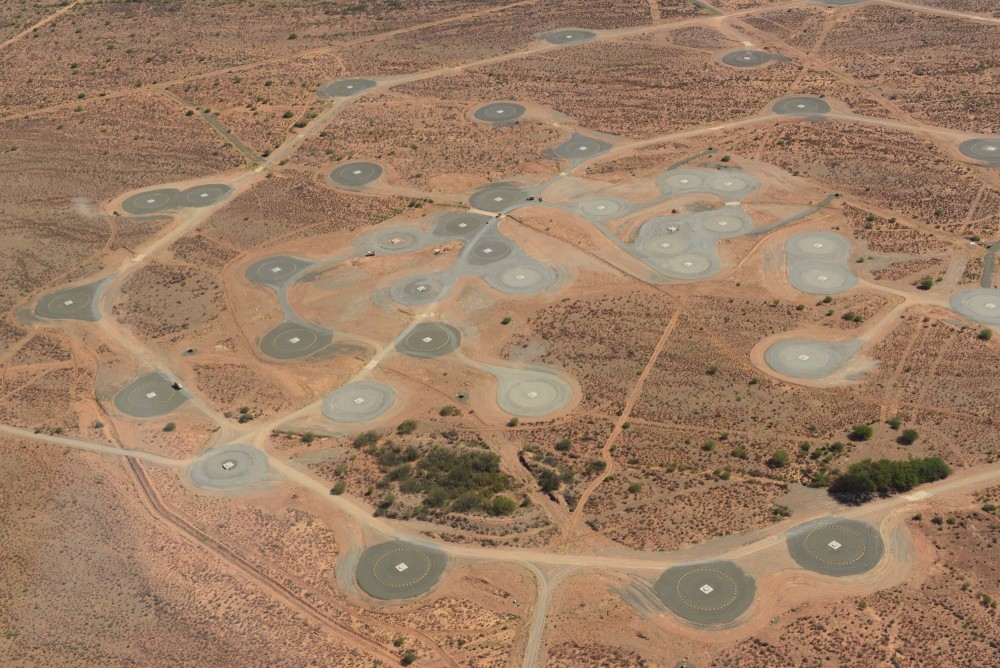
\includegraphics[width=0.9\textwidth]{mkat-core.jpg}
  \end{figure}
\end{frame}

\subsection{SPEAD}

\begin{frame}{High-performance Networking}
  \alert{S}treaming \alert{P}rotocol for \alert{E}xchange of
  \alert{A}stronomical \alert{D}ata
  \begin{itemize}
    \item Generic, not astronomy-specific at all
    \item Designed for moving numpy arrays around
    \item Used extensively in KAT-7 and MeerKAT
    \item Lossy one-way UDP transmission, multicast-friendly
  \end{itemize}
\end{frame}

\begin{frame}{Concepts}
  \begin{description}
    \item[Item] Data in a numpy array.
    \item[Heap] Unit of transmission. Contains multiple items.
    \item[Packet] UDP packet.
  \end{description}
  Heaps are broken down into multiple packets
\end{frame}

\begin{frame}{Example}
  Correlator heaps at \SI{2}{\Hz}:
  \begin{itemize}
    \item \texttt{xeng_raw} $8320\times 32768\times 2\times \text{int32}$
    \item \texttt{timestamp} int
  \end{itemize}
  Each \SI{2}{\gibi\byte} heap is split into \SI{9}{\kilo\byte} packets.

  \pause
  Total rate is \SI{35}{Gbps} / \SI{475}{Kpps}.

  \pause
  In reality, will split this into several streams.
\end{frame}

\begin{frame}{Not Your Average High-Speed Networking}
  \begin{itemize}
    \item Large packets (MTU 9200)
    \item Small number of flows
    \item Bandwidth matters, latency doesn't
  \end{itemize}
\end{frame}

\begin{frame}{Just To Make It Interesting}
  I had some goals:
  \begin{itemize}
    \item Run without root privileges
    \item Run on Linux and OS X
  \end{itemize}
\end{frame}

% Add a slide giving examples of how sensitive things are
\section{Talking to C++}

\subsection{An Example C++ Library}

\begin{frame}[fragile=singleslide]{Code}
\begin{lstlisting}[language=c++]
namespace petshop {

class Parrot {
    int volts;
public:
    void voom();
    void set_volts(int volts);
    int get_volts() const;
};

}
\end{lstlisting}
\end{frame}

\subsection{The Interface Zoo}

\begin{frame}[fragile]{Python C API}
  \begin{lstlisting}[language=c++,
    basicstyle=\ttfamily\supertiny,
    numberstyle=\supertiny,
    multicols=2]
#include "Python.h"
#include "petshop.h"
#include <memory>

typedef struct {
    PyObject_HEAD
    petshop::Parrot wrapped;
} Parrot;

static PyTypeObject ParrotType = {
    PyVarObject_HEAD_INIT(NULL, 0)
    "capi_petshop.Parrot"
};

static PyObject *
Parrot_new(PyTypeObject *type, PyObject *args, PyObject *kwds) {
    Parrot *self = (Parrot *) type->tp_alloc(type, 0);
    if (self != NULL)
    {
        new (&self->wrapped) petshop::Parrot();
    }
    return (PyObject *) self;
}

static void Parrot_dealloc(Parrot *self) {
    self->wrapped.~Parrot();
    Py_TYPE(self)->tp_free((PyObject *) self);
}

static PyObject *Parrot_voom(Parrot *self) {
    self->wrapped.voom();
    Py_RETURN_NONE;
}

static PyObject *Parrot_get_volts(Parrot *self, void *closure) {
    return PyLong_FromLong(self->wrapped.get_volts());
}

static int
Parrot_set_volts(Parrot *self, PyObject *value, void *closure) {
    long volts = PyLong_AsLong(value);
    if (PyErr_Occurred())
        return -1;
    if (volts < INT_MIN || volts > INT_MAX) {
        PyErr_SetString(PyExc_OverflowError,
            "Python int too large to convert to C int");
        return -1;
    }
    self->wrapped.set_volts(volts);
    return 0;
}

static PyMethodDef Parrot_methods[] = {
    {"voom", (PyCFunction) Parrot_voom, METH_NOARGS, "voom"},
    {NULL}
};

static PyGetSetDef Parrot_getseters[] = {
    {"volts", (getter) Parrot_get_volts,
              (setter) Parrot_set_volts, "volts", NULL},
    {NULL}
};

static struct PyModuleDef capi_petshop_module = {
    PyModuleDef_HEAD_INIT,
    "capi_petshop",
    NULL,
    -1,
    NULL,
};

extern "C" {

PyMODINIT_FUNC PyInit_capi_petshop(void) {
    PyObject *m;
    ParrotType.tp_new = Parrot_new;
    ParrotType.tp_basicsize = sizeof(Parrot);
    ParrotType.tp_flags = Py_TPFLAGS_DEFAULT;
    ParrotType.tp_dealloc = (destructor) Parrot_dealloc;
    ParrotType.tp_methods = Parrot_methods;
    ParrotType.tp_getset = Parrot_getseters;
    if (PyType_Ready(&ParrotType) < 0)
        return NULL;
    m = PyModule_Create(&capi_petshop_module);
    if (m == NULL)
        return NULL;
    Py_INCREF(&ParrotType);
    PyModule_AddObject(m, "Parrot", (PyObject *) &ParrotType);
    return m;
}
}
  \end{lstlisting}
  \pause
  \only<2>{%
    \begin{tikzpicture}[remember picture,overlay]
      \node at (current page.center) {\Huge \bfseries Just Say No};
    \end{tikzpicture}%
  }%
\end{frame}

\begin{frame}{Cython}{Overview}
  TODO: diagram of how Cython works
\end{frame}

\begin{frame}[fragile=singleslide]{Cython}{Definition File}
  \begin{lstlisting}[language=cython]
cdef extern from "petshop.h" namespace "petshop":
    cdef cppclass Parrot:
        void voom()
        void set_volts(int volts)
        int get_volts()
  \end{lstlisting}
\end{frame}

\begin{frame}[fragile=singleslide]{Cython}{Wrapper}
  \begin{lstlisting}[language=cython]
cimport c_petshop

cdef class Parrot:
    cdef c_petshop.Parrot _this

    def voom(self):
        self._this.voom()

    property volts:
        def __get__(self):
            return self._this.get_volts()

        def __set__(self, volts):
            self._this.set_volts(volts)
  \end{lstlisting}
\end{frame}

\begin{frame}[fragile=singleslide]{Cython}{Sometimes This Happens}
  \footnotesize
  \begin{verbatim}
Error compiling Cython file:
------------------------------------------------------------
...
    PyTypeObject *Py_TYPE(obj)
    bint PyMapping_Check(obj)
    object PyErr_Format(exc, const char *format, ...)

@cname("__pyx_convert__from_py_spead::in::item")
cdef item __pyx_convert__from_py_spead::in::item(obj) except *:
                                      ^
------------------------------------------------------------

FromPyStructUtility:11:39: Expected an identifier or literal
  \end{verbatim}
\end{frame}

\begin{frame}[fragile=singleslide]{Boost.Python}
  \begin{lstlisting}[language=c++]
#include <boost/python.hpp>
#include "petshop.h"

using namespace petshop;
using namespace boost::python;

BOOST_PYTHON_MODULE(bpy_petshop)
{
    class_<Parrot>("Parrot")
        .def("voom", &Parrot::voom)
        .add_property("volts",
            &Parrot::get_volts, &Parrot::set_volts);
}
  \end{lstlisting}
\end{frame}

\begin{frame}{Sir-Not-Appearing-In-These-Slides}
  SWIG
  \begin{itemize}
    \item Targets many languages, not just Python
    \item Understands C++ and templates
    \item Compiles to Python C API
    \item Quick glance at docs look promising!
  \end{itemize}
  cffi
  \begin{itemize}
    \item C only
    \item Recommended for PyPy support
  \end{itemize}
  ctypes
  \begin{itemize}
    \item Also C only
    \item No compilation step, ABI-level only
  \end{itemize}
\end{frame}

\begin{frame}{Interface Summary}
  \def\yes{\textcolor{green!50!black}{\CheckmarkBold}}
  \def\no{\textcolor{red}{\XSolidBrush}}
  \begin{table}
    \begin{tabular}{lcccc}
      \toprule
      Interface & C++ & PyPy & No new lang & Runtime\\
      \midrule
      C API & \no & \no & \yes & ---\\
      cffi  & \no & \yes & \yes & cffi\\
      Cython & \yes & \no & \no & ---\\
      Boost.Python & \yes & \no & \yes & Boost\\
      ctypes & \no & (\yes) & \yes & ---\\
      SWIG & \yes & \no & \no & ?\\
      \bottomrule
    \end{tabular}
  \end{table}
\end{frame}

% - The problem
%   - MeerKAT
%   - SPEAD
%   - High performance networking, but different
% - The approach
%   - Why Python
%     - we're a Python shop; protocol is based on numpy
%   - Why C++ (and how hard is it really?)
% - Possible solutions
%   - Pure Python
%   - ctypes, cffi
%   - Cython
%     - Show the compiler error
%   - Python C API
%     - Yuck!
%   - Boost.Python
%     - Show a noddy example
%     - Downside: a runtime system library dependency
% - The interesting stuff
%   - GIL
%     - GIL background
%   - Lifetime management (custodian and ward)
%   - KeyboardInterrupt
%   - asyncio
%   - logging
%   - exceptions
%   - bytestring conversion

\section{Boost.Python}

\begin{frame}<beamer>{Outline}
  \tableofcontents[currentsection]
\end{frame}

\begin{frame}{Easy Things Are Easy}
  \begin{itemize}
    \item Keyword and default arguments
    \item Exception mapping
    \item Operator overloads
  \end{itemize}
\end{frame}

\subsection[GIL]{Global Interpreter Lock}

\begin{frame}{Why do we care?}
  \begin{itemize}
    \item Waiting for a heap should not block other threads
    \item Non-Python threads calling Python code
  \end{itemize}
\end{frame}

\begin{frame}[fragile=singleslide]{Releasing the GIL, C++-style}
  \begin{lstlisting}[language=c++]
class release_gil {
    PyThreadState *save;
public:
    release_gil() {
        save = PyEval_SaveThread();
    }

    ~release_gil() {
        PyEval_RestoreThread(save);
    }
};
  \end{lstlisting}
\end{frame}

\begin{frame}[fragile=singleslide]{Acquiring the GIL, C++ style}
  \begin{lstlisting}[language=c++]
class acquire_gil {
    PyGILState_STATE gstate;
public:
    acquire_gil() {
        gstate = PyGILState_Ensure();
    }

    ~acquire_gil() {
        PyGILState_Release(gstate);
    }
};
  \end{lstlisting}
\end{frame}

\subsection{Unicode}

\begin{frame}{Quick Reminder}
  \centering
  \begin{tabular}{ccl}
    \toprule
    \textbf{Python 2} & \textbf{Python 3} & \textbf{Purpose}\\
    \midrule
    \linlinep"str" / \linlinep"bytes" & \linlinep"bytes" & Encoded byte sequence\\
    \linlinep"unicode" & \linlinep"str" & Unicode code points\\
    \bottomrule
  \end{tabular}
\end{frame}

\begin{frame}{What Would Boost.Python Do?}
  \begin{description}
    \item[Python 2] \linlinep"str" $\leftrightarrow$ \linlinec"std::string"
    \item[Python 3] \linlinep"str" $\leftrightarrow$ \linlinec"std::string", UTF-8\\
                    \linlinep"bytes" $\rightarrow$ \linlinec"std::string"
  \end{description}
  \pause
  What if I want \linlinec"std::string" $\rightarrow$ \linlinep"bytes"?
\end{frame}

\begin{frame}[fragile=singleslide]{Custom Converters}
We'll define a new C++ class for this.
  \begin{lstlisting}[language=c++]
class bytestring : public std::string {
{
public:
    using std::string::string;

    bytestring(const std::string &s)
        : std::string(s) {}
    bytestring(std::string &&s)
        : std::string(std::move(s)) {}
};
  \end{lstlisting}

This is just a class interchangeable with \linlinec"std::string".
\end{frame}

\begin{frame}[fragile=singleslide]{Custom Converters}
  Define how to convert it to Python:
  \begin{lstlisting}[language=c++]
class bytestring_to_python
{
public:
    static PyObject *convert(const bytestring &s)
    {
        return PyBytes_FromStringAndSize(
            s.data(), s.size());
    }
};
  \end{lstlisting}
  {\footnotesize (only Python 3 version shown)}
\end{frame}

\begin{frame}[fragile=singleslide]{Custom Converters}
  \alert{Register} the converter
  \begin{lstlisting}[language=c++]
to_python_converter<bytestring, bytestring_to_python>();
  \end{lstlisting}
\end{frame}

\subsection{Object Lifetime}

\begin{frame}{Reminder}
  In CPython, objects have a \alert{reference count}.
  \begin{itemize}
    \item Increment it to hold a reference.
    \item Decrement it to drop the reference.
    \item When it hits zero, object is deleted.
  \end{itemize}
  Very easy to screw up with Python C API.
\end{frame}

\begin{frame}{C++ To The Rescue}
  \linlinec"boost::python::handle" is a smart wrapper
  \begin{itemize}
    \item Copy constructor increments the refcount
    \item Destructor decrements the refcount
  \end{itemize}

  \pause
  \alert{Caution}: not safe while \linlinec{release_gil} active
\end{frame}

\begin{frame}[fragile=singleslide]{Putting Things On Top Of Other Things}
  What about C++ objects referencing other C++ objects?
  \begin{lstlisting}[language=c++]
class flowers {
public:
    string name;
    explicit flowers(const string &name) : name(name) {}
};

class vase {
    flowers *contents = nullptr;
public:
    void set_contents(flowers &value) {
        contents = &value;
    }

    string str() const {
        return (contents ? contents->name : "empty");
    }
};
  \end{lstlisting}
\end{frame}

\begin{frame}[fragile]{Na{\"\i}ve Wrapping}
  \begin{lstlisting}[language=c++]
BOOST_PYTHON_MODULE(custodian1) {
    using namespace boost::python;
    class_<flowers>("Flowers", init<string>());
    class_<vase>("Vase")
        .def("set_contents", &vase::set_contents)
        .def("__str__", &vase::str);
}
  \end{lstlisting}
  \pause
  \begin{lstlisting}[language=python,numbers=none]
>>> from custodian1 import *
>>> v = Vase()
>>> str(v)
'empty'
>>> v.set_contents(Flowers('tulips'))
>>> str(v)
Segmentation fault
  \end{lstlisting}
\end{frame}

\begin{frame}[fragile=singleslide]{Custodians And Wards}
  Let's tell Boost.Python about the relationship:
  \begin{lstlisting}[language=c++]
BOOST_PYTHON_MODULE(custodian) {
    using namespace boost::python;
    class_<flowers>("Flowers", init<string>());
    class_<vase>("Vase")
        .def("set_contents", &vase::set_contents,
            with_custodian_and_ward_postcall<1, 2>())
        .def("__str__", &vase::str);
}
  \end{lstlisting}
\end{frame}

\begin{frame}{Custodians And Wards}
  What Happened?

  TODO: picture of the nurse and patient
\end{frame}

\begin{frame}[fragile=singleslide]{Help, My Python Is Leaking!}
  What Happens Here?
  \begin{lstlisting}[language=python]
v = Vase()
for line in sys.stdin:
    v.set_contents(Flowers(line))
  \end{lstlisting}
\end{frame}

\begin{frame}[fragile=singleslide]{Backreferences}
  Let's try another approach:
  \begin{lstlisting}[language={[extra]c++}]
class flowers {
public:
    $PyObject *self;$
    string name;
    flowers($PyObject *self$, const string &name)
        : $self(self)$, name(name) {}
};

class vase {
    flowers *contents = nullptr;
    $handle<> ref;$
public:
    void set_contents(flowers &value) {
        contents = &value;
        $ref = handle<>(borrowed(value.self));$
    }
    ...
};
  \end{lstlisting}
\end{frame}

\begin{frame}[fragile=singleslide]{Backreferences}
  To make Boost.Python use the new constructor:
  \begin{lstlisting}[language={[extra]C++}]
BOOST_PYTHON_MODULE(backref) {
    class_<flowers, $flowers, boost::noncopyable$>(
        "Flowers", init<string>());
    class_<vase>("Vase")
        .def("set_contents", &vase::set_contents)
        .def("__str__", &vase::str);
}
  \end{lstlisting}
\end{frame}

\section*{Summary}

\begin{frame}[<+->]{Summary}{The Good}
  \begin{itemize}
    \item Fantastic for integrating C++ classes
    \item Can drop down to Python C API when needed
    \item No new language to learn
  \end{itemize}
\end{frame}

\begin{frame}[<+->]{Summary}{The Not So Good}
  \begin{itemize}
    \item Introduces a system library dependency
    \item Lots of deep metaprogramming magic
    \item Doesn't support PyPy\footnote{as far as I know}
  \end{itemize}
\end{frame}

\end{document}
